\documentclass[11pt]{article}

\usepackage[margin=1.5in]{geometry}
\usepackage{amsmath, amssymb, amsthm, mathrsfs}
\usepackage{lmodern, inconsolata}
\usepackage{secdot, sectsty}
\usepackage{secdot}
\usepackage{bbm}
\usepackage{fancyhdr}
\usepackage{caption, graphicx}
\usepackage{listings}
\usepackage{color}
\usepackage{enumitem}
\usepackage{booktabs, threeparttable, adjustbox, tabularx, longtable}
\usepackage{hyperref}
\usepackage{soul}
\usepackage{float}

\newcommand{\inv}[1]{#1^{-1}}
\newcommand{\iid}{\text{i.i.d.}}
\newcommand{\bmat}[1]{\begin{bmatrix} #1 \end{bmatrix}}
\newcommand{\asconv}{\xrightarrow{a.s.}}
\newcommand{\pconv}{\xrightarrow{p}}
\newcommand{\dconv}{\xrightarrow{d}}
\newcommand{\msconv}{\xrightarrow{m.s.}}
\newcommand{\liminfty}{\lim_{n \to \infty}}
\newcommand*\diff{\mathop{}\!\mathrm{d}}
\newcommand{\lhood}{\mathcal{L}}
\renewcommand{\vec}[1]{\mathbf{#1}}

\newtheorem*{proposition}{Proposition}
\newtheorem*{claim}{Claim}

\let\oldforall\forall
\let\forall\undefined
\DeclareMathOperator{\forall}{\oldforall}
\DeclareMathOperator{\ev}{E}
\DeclareMathOperator{\var}{Var}
\DeclareMathOperator*{\argmax}{arg\,max}
\DeclareMathOperator*{\argmin}{arg\,min}

\lstset{
  basicstyle=\footnotesize\ttfamily,
  columns=fixed,
  fontadjust=true,
  basewidth=0.5em
}

\sectionfont{\normalsize}
\subsectionfont{\normalsize\selectfont}
\subsubsectionfont{\normalsize\selectfont}

\sectiondot{subsection}

\newcommand{\specialcell}[2][c]{\begin{tabular}[#1]{@{}c@{}}#2\end{tabular}}

\usepackage[backend=bibtex, style=authortitle, citestyle=authoryear-icomp, url=false]{biblatex}
\addbibresource{citations.bib}

\linespread{1}

\begin{document}

\title{Heterogeneous Spillovers in Unconditional Cash Transfers}

\author{
	Justin Abraham, Nathaniel Bechhofer, Minki Kim
}

\maketitle

	\begin{abstract}

		In an unconditional cash transfer (UCT) program conducted in rural Kenya, \textcite{haushofer_short-term_2016} report that villages where households were given transfers saw even those who did not receive transfers obtain spillover benefits, as they can compare non-treated villagers in the treatment villages to those in the control villages. We test if the within-village spillover effects from unconditional cash transfer vary by demographic characteristics. Our findings suggest that even though the spillovers are on average beneficial to those who did not receive the transfer, those who are demographically dissimilar to average villagers might have experienced negative spillovers, both in pecuniary and non-pecuniary measures.

 	\end{abstract}

\section{Introduction}

    \textcite{haushofer_short-term_2016} demonstrate that villages where villagers were given transfers saw even those who did not receive transfers obtain spillover benefits, as they can compare non-treated villagers in the treatment villages to those in the control villages. We allow for these spillovers to vary by demographics, as we might expect that villagers similar to recipients of the cash transfers would enjoy more spillover benefits.


\section{Data}

    This analysis will use data from a randomized controlled trial of an unconditional cash transfer (UCT) program conducted in rural Kenya \parencite{haushofer_short-term_2016}. Between 2011 and 2013, GiveDirectly provided UCTs to poor households\footnote{At the time eligibility for the program was determined by living in a house with a thatched roof.} in rural Kenya amounting to USD PPP 404 and USD PPP 1525. The experimental design involved the random assignment of 60 villages to participate in the program and 60 in the control group \textit{and} the random assignment of eligible households within treatment villages to receive a cash transfer. Among households receiving the transfer, the trial also randomized whether the recipient was the head male or female, whether the transfer was paid out regularly or in a lump sum, and the size of the transfer. The data is comprised of a baseline survey collected before the intervention ($N=1008$), an endline survey a few weeks after the end of the intervention ($N=940$), and a long-term follow up 3 years after the endline survey ($N=901$). Surveys collected for sample households information on asset ownership, consumption, education, physical health, subjective well-being, business activity, labor supply, political behavior, investment decisions, and cortisol levels. The baseline and endline survey also collected village-level data on prices, wages, and violent conflict.

\section{Empirical Strategy}

    \subsection{Selection among the pure control villages}

        A potential concern for the estimation strategy we lay out in this section is that in the original experiment the thatched-roof selection criterion was applied to the pure control villages one year after it was applied to households in the treated villages. Thus, pure control households that upgraded their roofs during this one-year span would have been excluded from the sample, allowing for the possibility of selection bias. We follow the strategy outlined in \textcite{haushofer_short-term_2016} to address this issue by testing whether pure control households differ from the originally sampled households on a set of immutable characteristics--those variables that remain constant during the time between samples.\footnote{These variables are age of the primary respondent, marital status of the primary respondent, highest level of education, the number of children excluding those born between baseline and endline, and the household size at baseline.}\footnote{We refer readers to \textcite{haushofer_short-term_2016} for additional robustness checks including prediction of roof upgrades, treatment effect bounds, and resurveys of the pure control group.} Another concern with the data is that it lacks baseline characteristics for the control villages. Nevertheless, we can still estimate \textit{differences} in spillover effects by exclusively looking at non-treated villagers in the treatment villages and imputing deviations from the endline mean for the control group. This does come with the limitation that we cannot rule out demographic differences in trends that would occur regardless of whether villagers lived in villages that were treated.

    \subsection{Linear spillover effects}

        To test whether similarity to treated households results in differential spillover effects, we estimate a parsimonious model that interacts a measure of demographic distance $D_{i,v}$ with an indicator for living in a treatment village $S_v$.

            \begin{equation} \label{eq:interaction}
            Y_{i,v} = \beta_0 + \beta_1 S_v + \beta_2 D_{i,v} + \beta_3 S_v \times  D_{i,v} + \varepsilon_{i,v}
            \end{equation}

        $Y_{i,v}$ is the outcome variable of interest with households indexed by $i$ in village $v$.\footnote{For comparability with the original experiment, we estimate Eq. \ref{eq:interaction} using the same set of outcome variables: the value of non-land assets, non-durable expenditures, monthly household revenue, and indices of food security, health, education, subjective well-being, and female empowerment. We estimate the eight equations simultaneously to allow for cross-correlations and to be able to conduct joint tests.} $D_{i,v}$ is a measure of distance of each household from characteristics of treatment households. $\varepsilon_{i,v}$ is the idiosyncratic error term. Standard errors are clustered at the village level. Since village treatment status was randomly assigned, $\beta_1 + \beta_3 D_{i,v}$ can be interpreted as the marginal effect on $Y_{i,v}$ of living in a village in which some households receive cash transfers. We test the null hypothesis $\beta_3 = 0$: that the spillover effect does not depend on distance.

        Our first measure of demographic distance uses the pre-treatment levels of each respective outcome and denoted by $Y_{i,v,t=0}$. We calculate a normalized absolute distance from the village-specific average of the treated households.\footnote{As discussed in the previous section, we impute baseline characteristics of the pure control households from the endline survey and argue that they remain comparable to the spillover households on average.}

            \begin{equation} \label{eq:absdev}
            D_{i,v} = \frac{|Y_{i,v,t=0} - \bar Y_{v,t=0}|}{\text{SD}_v}
            \end{equation}

        % Additionally, we calculate squared deviations from village averages.
        %
        %     \begin{equation} \label{eq:sqdev}
        %     D^2_{i,v} = \frac{(Y_{i,v,t=0} - \bar Y_{v,t=0})^2}{\text{SD}_v}
        %     \end{equation}

        This specifications assumes that only the baseline level of the outcomes moderates the spillover effects of the cash transfers. To allow a more general model that lets effects differ along multiple observables, we estimate Eq. \ref{eq:interaction} with a Mahalanobis measure $D^\text{M.}_{i,v}$. Let $\mathbf X_i$ denote the vector of household-level observables and $\mathbf{\bar X}$ the village-specific sample means of treated households. $\mathbf{\hat S}_v$ is the village-specific covariance. We include the pre-treatment levels of each outcome variable as well as a set of covariates listed in \textcite{haushofer_short-term_2016}.

            \begin{equation} \label{eq:mdist}
            D^\text{M.}_{i,v} = \sqrt{(\mathbf X_i - \mathbf{\bar X})' \mathbf{\hat S}^{-1}_v (\mathbf X_i - \mathbf{\bar X})}
            \end{equation}

        This measure allows us to calculate a univariate metric of demographic distance that accounts for correlations between characteristics.

    \subsection{Non-linear spillover effects}

        We further generalize the model by allowing for non-linearities in the distance term.

\section{Results}

    \begin{table}[H]
    \centering
    \caption{Balance on immutable characteristics}
    \label{tab:balance}
    \maxsizebox*{\textwidth}{\textheight}{
    \begin{threeparttable}
    {
\def\sym#1{\ifmmode^{#1}\else\(^{#1}\)\fi}
\begin{tabular}{l*{3}{SSSSS}}
\toprule
          &\multicolumn{1}{c}{(1)}&\multicolumn{1}{c}{(2)}&\multicolumn{1}{c}{(3)}\\
          &\multicolumn{1}{c}{\specialcell{Treatment Village\\Mean (SD)}}&\multicolumn{1}{c}{\specialcell{Control Village\\Mean (SD)}}&\multicolumn{1}{c}{\specialcell{Difference}}\\
\midrule
Age (respondent)&    35.35&    34.84&    -0.51\\
          &  (14.13)&  (14.31)&   (0.95)\\
Marital status (respondent)&     0.78&     0.75&    -0.04\\
          &   (0.41)&   (0.44)&   (0.03)\\
Number of children&     2.88&     2.84&    -0.04\\
          &   (1.91)&   (1.92)&   (0.15)\\
Household size&     4.94&     4.75&    -0.19\\
          &   (2.16)&   (2.23)&   (0.17)\\
Years of education completed (respondent)&     8.53&     8.73&     0.19\\
          &   (2.95)&   (3.00)&   (0.20)\\
\midrule Joint test (\emph{p}-value)&         &         &0.08$^{*}$\\
\bottomrule
\end{tabular}
}

    \begin{tablenotes}[flushleft] \footnotesize \item \emph{Notes}: Estimates of the mean of immutable baseline characteristics calculated among households in treatment
    villages and control villages. Baseline characteristics are listed on the left. Column (1) reports the mean (std. dev.) taken among households in treatment villages.  Column (2) reports the mean (std. dev.) taken among households in control villages. Column (3) reports the difference in means calculated using an OLS regression of the baseline characteristic on an indicator variable for living in a treatment village. Village-level clustered standard errors are reported in parentheses. The last row reports a test of joint significance after estimation using SUR. * denotes significance at 10 pct., ** at 5 pct., and *** at 1 pct. level.
    \end{tablenotes}
    \end{threeparttable}
    }
    \end{table}

    Table \ref{tab:balance} reports balance across treatment and control villages on immutable characteristics of households. As in the original study, we fail to reject a joint test of balance between transfer and control villages across all variables at the 5 percent level. Table \ref{tab:absdev} shows the heterogenous spillover effects on various dependent variables, using the absolute deviation as a measure of demographic distance. In the first column, we report the effects of one standard deviation increase in absolute distance  $D_i^{Abs.}$ on the spillover effects. For all dependent variables, we found evidence of negative relations between demographic distance and spillover effects. The signs of the coefficients for the interaction terms are the opposite of those for the spillover dummy terms. \\

    \begin{table}[H]
    \centering
    \caption{Spillover effects by absolute distance from village means}
    \label{tab:absdev}
    \maxsizebox*{\textwidth}{\textheight}{
    \begin{threeparttable}
    {
\def\sym#1{\ifmmode^{#1}\else\(^{#1}\)\fi}
\begin{tabular}{l*{5}{c}}
\toprule
          &\multicolumn{1}{c}{Interaction}&\multicolumn{1}{c}{Abs. distance}&\multicolumn{1}{c}{\specialcell{Treated village}}&\multicolumn{1}{c}{\specialcell{Control mean\\(Std. dev.)}}&\multicolumn{1}{c}{Obs.}\\
\midrule
\midrule Value of non-land assets (USD)&-111.103$^{***}$&203.299$^{***}$&92.200$^{**}$&   384.05&      901\\
          & (41.440)& (31.743)& (37.393)& (298.69)&         \\
Non-durable expenditure (USD)&-49.941$^{***}$&52.684$^{***}$&32.360$^{***}$&   165.38&      901\\
          & (10.184)&  (6.917)&  (9.504)&  (90.90)&         \\
Total revenue, monthly (USD)&-68.286$^{***}$&98.174$^{***}$&48.735$^{***}$&    52.66&      901\\
          & (17.755)& (11.947)& (11.143)&  (95.22)&         \\
Food security index&0.473$^{***}$&-0.628$^{***}$&-0.307$^{**}$&    -0.06&      901\\
          &  (0.166)&  (0.140)&  (0.129)&   (1.26)&         \\
Health index&   -0.059&   -0.015&    0.000&     0.06&      901\\
          &  (0.153)&  (0.117)&  (0.121)&   (1.06)&         \\
Education index&    0.158&    0.035&   -0.055&    -0.01&      750\\
          &  (0.167)&  (0.122)&  (0.122)&   (1.03)&         \\
Psychological well-being index&    0.066&    0.014&   -0.022&    -0.03&     1396\\
          &  (0.103)&  (0.078)&  (0.102)&   (0.98)&         \\
Female empowerment index&0.913$^{***}$&-0.917$^{***}$&-0.513$^{***}$&    -0.21&      661\\
          &  (0.155)&  (0.109)&  (0.129)&   (1.15)&         \\
\bottomrule
\end{tabular}
}

    \begin{tablenotes}[flushleft] \footnotesize \item \emph{Notes}:
    The unit of observation is the household for all outcome variables except for the psychological variables index, where it is the individual. The sample is restricted to co-habitating couples for the female empowerment index, and households with school-age children for the education index. All columns include village-level fixed effects, control for baseline outcomes, and cluster standard errors at the village level. * denotes significance at 10 pct., ** at 5 pct., and *** at 1 pct. level.
    \end{tablenotes}
    \end{threeparttable}
    }
    \end{table}

    For all five dependent variables with statistically significant baseline spillover effects, the effects of one standard deviation increase in the absolute distance were more than enough to completely offset the baseline spillover effects. For instance, households one standard deviation away from the mean demographic characteristic of the village they belong to experienced (on average) a \textit{negative} spillover effects on total revenue, which amount to -19.5 USD. We found no significant heterogenous spillover effects on food security, health, and education indices.

    In Table \ref{tab:sqdev} we report the results from the same regressions, this time with the squared distances $D_i^2$ as a measure of demographic distance. Once again, the results strongly indicate that households dissimilar from an average villager experienced weaker spillover effects. The magnitude of the coefficients of the interaction terms are smaller, because the squared distance measure weights distances far away from the mean more heavily.

    % \begin{table}[H]
    % \centering
    % \caption{Spillover effects by squared distance from village means}
    % \label{tab:sqdev}
    % \maxsizebox*{\textwidth}{\textheight}{
    % \begin{threeparttable}
    % {
\def\sym#1{\ifmmode^{#1}\else\(^{#1}\)\fi}
\begin{tabular}{l*{5}{c}}
\toprule
          &\multicolumn{1}{c}{Interaction}&\multicolumn{1}{c}{Sq. distance}&\multicolumn{1}{c}{\specialcell{Treated village}}&\multicolumn{1}{c}{\specialcell{Control mean\\(Std. dev.)}}&\multicolumn{1}{c}{Obs.}\\
\midrule
\midrule Value of non-land assets (USD)&-0.436$^{***}$&0.550$^{***}$&94.834$^{***}$&   384.05&      901\\
          &  (0.052)&  (0.043)& (21.403)& (298.69)&         \\
Non-durable expenditure (USD)&-0.434$^{***}$&0.472$^{***}$&21.569$^{***}$&   165.38&      901\\
          &  (0.036)&  (0.025)&  (7.409)&  (90.90)&         \\
Total revenue, monthly (USD)&-0.470$^{***}$&0.499$^{***}$&24.317$^{***}$&    52.66&      901\\
          &  (0.018)&  (0.017)&  (4.650)&  (95.22)&         \\
Food security index&0.310$^{***}$&-0.419$^{***}$&-0.279$^{***}$&    -0.06&      901\\
          &  (0.061)&  (0.031)&  (0.085)&   (1.26)&         \\
Health index&    0.023&   -0.052&   -0.068&     0.06&      901\\
          &  (0.099)&  (0.077)&  (0.092)&   (1.06)&         \\
Education index&   -0.034&0.215$^{***}$&    0.086&    -0.01&      750\\
          &  (0.096)&  (0.080)&  (0.091)&   (1.03)&         \\
Psychological well-being index&    0.052&    0.003&   -0.017&    -0.03&     1396\\
          &  (0.068)&  (0.060)&  (0.086)&   (0.98)&         \\
Female empowerment index&0.406$^{***}$&-0.424$^{***}$&-0.217$^{**}$&    -0.21&      661\\
          &  (0.055)&  (0.019)&  (0.091)&   (1.15)&         \\
\bottomrule
\end{tabular}
}

    % \begin{tablenotes}[flushleft] \footnotesize \item \emph{Notes}:
    % The unit of observation is the household for all outcome variables except for the psychological variables index, where it is the individual. The sample is restricted to co-habitating couples for the female empowerment index, and households with school-age children for the education index. All columns include village-level fixed effects, control for baseline outcomes, and cluster standard errors at the village level. * denotes significance at 10 pct., ** at 5 pct., and *** at 1 pct. level.
    % \end{tablenotes}
    % \end{threeparttable}
    % }
    % \end{table}

    % \begin{table}[H]
    % \centering
    % \caption{Quadratic spillover effects}
    % \label{tab:quadratic}
    % \maxsizebox*{\textwidth}{\textheight}{
    % \begin{threeparttable}
    % {
\def\sym#1{\ifmmode^{#1}\else\(^{#1}\)\fi}
\begin{tabular}{l*{5}{c}}
\toprule
          &\multicolumn{1}{c}{\specialcell{Treated $\times$\\ Abs. distance}}&\multicolumn{1}{c}{\specialcell{Treated $\times$\\ Sq. distance}}&\multicolumn{1}{c}{\specialcell{Treated village}}&\multicolumn{1}{c}{\specialcell{Control mean\\(Std. dev.)}}&\multicolumn{1}{c}{Obs.}\\
\midrule
Value of non-land assets (USD)&259.86\sym{**}&-199.01\sym{***}&   -24.93&   384.05&      899\\
          & (104.17)&  (52.67)&  (42.69)& (298.69)&         \\
Non-durable expenditure (USD)&63.26\sym{**}&-63.43\sym{***}&    -2.36&   165.38&      899\\
          &  (31.59)&  (16.01)&  (12.34)&  (90.90)&         \\
Total revenue, monthly (USD)&102.51\sym{***}&-77.61\sym{***}&   -13.32&    52.66&      899\\
          &  (34.62)&  (14.92)&  (13.23)&  (95.22)&         \\
Food security index&-1.58\sym{***}&1.07\sym{***}&     0.27&    -0.06&      899\\
          &   (0.47)&   (0.26)&   (0.18)&   (1.26)&         \\
Health index&    -0.40&     0.21&     0.06&     0.06&      899\\
          &   (0.49)&   (0.28)&   (0.16)&   (1.06)&         \\
Education index&     0.30&    -0.20&    -0.06&    -0.01&      724\\
          &   (0.58)&   (0.35)&   (0.16)&   (1.03)&         \\
Psychological well-being index&     0.07&    -0.01&    -0.02&    -0.19&     1321\\
          &   (0.35)&   (0.20)&   (0.13)&   (0.94)&         \\
Female empowerment index&-0.74\sym{**}&0.78\sym{***}&     0.04&    -0.21&      621\\
          &   (0.36)&   (0.16)&   (0.14)&   (1.15)&         \\
\bottomrule
\end{tabular}
}

    % \begin{tablenotes}[flushleft] \footnotesize \item \emph{Notes}:
    % The unit of observation is the household for all outcome variables except for the psychological variables index, where it is the individual. The sample is restricted to co-habitating couples for the female empowerment index, and households with school-age children for the education index. All columns include village-level fixed effects, control for baseline outcomes, and cluster standard errors at the village level. * denotes significance at 10 pct., ** at 5 pct., and *** at 1 pct. level.
    % \end{tablenotes}
    % \end{threeparttable}
    % }
    % \end{table}

    \begin{table}[H]
    \centering
    \caption{Spillover effects by Mahalanobis distance from village means}
    \label{tab:mahalanobis}
    \maxsizebox*{\textwidth}{\textheight}{
    \begin{threeparttable}
    {
\def\sym#1{\ifmmode^{#1}\else\(^{#1}\)\fi}
\begin{tabular}{l*{5}{c}}
\toprule
          &\multicolumn{1}{c}{Interaction}&\multicolumn{1}{c}{\specialcell{Treated village}}&\multicolumn{1}{c}{\(D^\text{M.}\)}&\multicolumn{1}{c}{\specialcell{Control mean\\(Std. dev.)}}&\multicolumn{1}{c}{Obs.}\\
\midrule
Value of non-land assets (USD)&   -22.68&    82.08&    11.21&   384.05&      519\\
          &  (43.14)& (141.67)&  (38.66)& (298.69)&         \\
Non-durable expenditure (USD)&    11.69&   -26.23&-23.54\sym{**}&   165.38&      519\\
          &  (12.66)&  (42.87)&  (11.42)&  (90.90)&         \\
Total revenue, monthly (USD)&    -4.03&     5.77&    10.03&    52.66&      519\\
          &  (10.13)&  (32.61)&   (9.15)&  (95.22)&         \\
Food security index&     0.07&    -0.36&     0.00&    -0.06&      519\\
          &   (0.12)&   (0.41)&   (0.11)&   (1.26)&         \\
Health index&     0.09&    -0.30&-0.17\sym{*}&     0.06&      519\\
          &   (0.11)&   (0.37)&   (0.09)&   (1.06)&         \\
Education index&0.28\sym{**}&-0.76\sym{*}&-0.22\sym{**}&    -0.01&      508\\
          &   (0.12)&   (0.41)&   (0.11)&   (1.03)&         \\
Psychological well-being index&     0.07&    -0.30&     0.01&    -0.19&      891\\
          &   (0.11)&   (0.37)&   (0.09)&   (0.94)&         \\
Female empowerment index&0.52\sym{***}&-1.47\sym{***}&-0.46\sym{***}&    -0.21&      484\\
          &   (0.16)&   (0.53)&   (0.14)&   (1.15)&         \\
\bottomrule
\end{tabular}
}

    \begin{tablenotes}[flushleft] \footnotesize \item \emph{Notes}:
    The unit of observation is the household for all outcome variables except for the psychological variables index, where it is the individual. The sample is restricted to co-habitating couples for the female empowerment index, and households with school-age children for the education index. All columns include village-level fixed effects, control for baseline outcomes, and cluster standard errors at the village level. * denotes significance at 10 pct., ** at 5 pct., and *** at 1 pct. level.
    \end{tablenotes}
    \end{threeparttable}
    }
    \end{table}

    \begin{figure}[ht]
    \centering
    \caption{Quadratic spillover effects by demographic distance}
    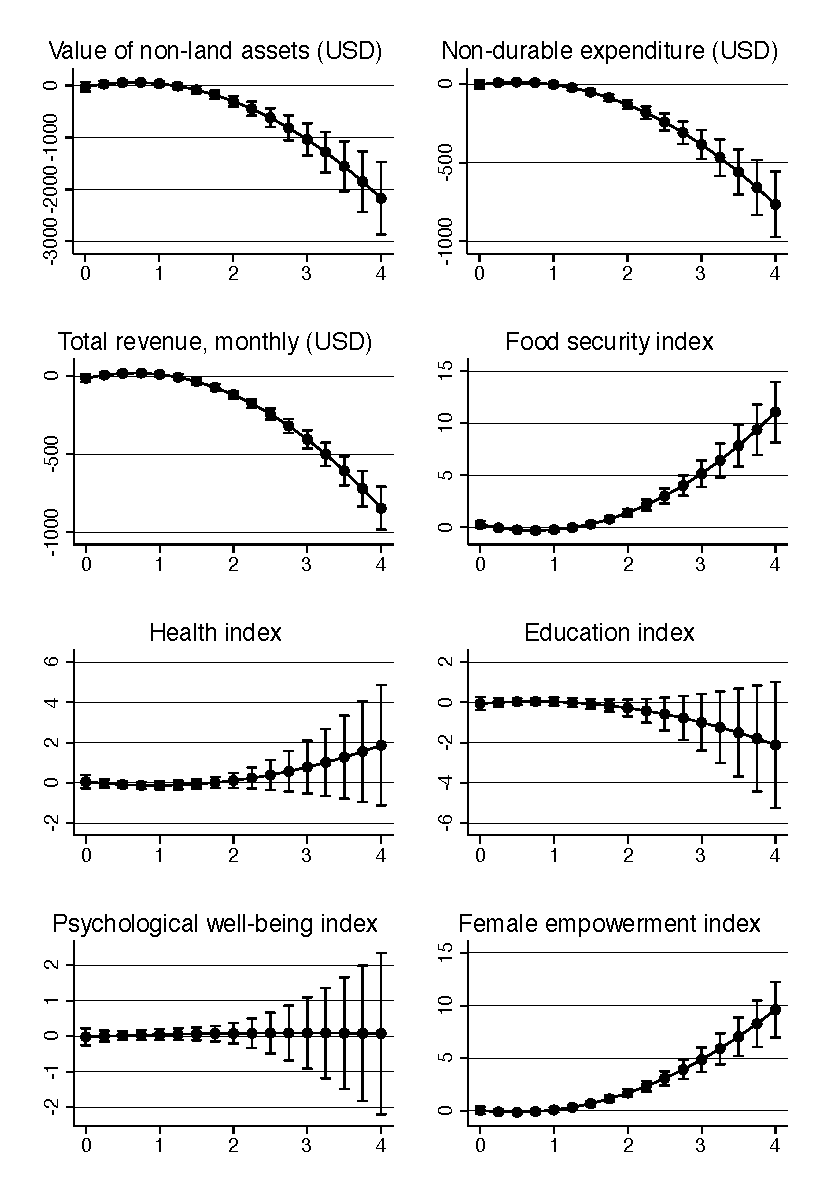
\includegraphics[height=0.85\textheight]{../Figs/indices_ppp_margins.pdf}
    \label{fig:margins}
    \caption*{\footnotesize \emph{Notes:} }
    \end{figure}

\section{Conclusion}

    We tested if within-village spillover effects from unconditional cash transfer vary by demographic characteristics. In an unconditional cash transfer (UCT) program conducted in rural Kenya, \textcite{haushofer_short-term_2016} found out that villages where villagers were given transfers saw even those who did not receive transfers obtain spillover benefits, as they can compare non-treated villagers in the treatment villages to those in the control villages. Our findings suggest that even though the spillovers are on average positive, those who are demographically dissimilar to other villagers might have experienced negative spillovers, both in pecuniary and non-pecuniary measures.


\newpage

\printbibliography

\end{document}
